% ============================================================
% Chapter 17 — Cost Analysis & the Bridge to Project II
% Folder: chapters/17-cost-bridge
% Course: Project Planning & Prototyping (247-519-VA, Vanier College)
% ============================================================

\chapter{Cost Analysis \& the Bridge to Project~II}
\label{ch17}

\paragraph{Where this fits.}
Chapter~16 assembled the complete documentation package --- the Design History
File, test reports, and version-controlled artefacts that constitute the
prototype record.
This final chapter adds the two pieces that convert a documented prototype
into a fundable project: a production economics analysis and a Gate~3
readiness statement.
Together they answer the gate committee's hardest question --- not ``does it
work?'' but ``can it be made and sold profitably, and is the risk of
proceeding lower than the risk of stopping?''

\paragraph{Learning Objectives.}
After completing this chapter you will be able to:
\begin{enumerate}
  \item Project unit cost at three production volumes using the cost model
        established in Chapter~12.
  \item Compute the revenue break-even volume and gross margin at a target
        price.
  \item Compute total profit at a given volume.
  \item Articulate Gate~3 readiness: what was proven, what remains, and why
        proceeding is economically justified.
\end{enumerate}

Every engineering team that reaches Gate~3 has built something that works.
The sorting subsystem sorts, the AI inference runs, the bracket holds.
The harder question --- the one the gate committee is paid to ask --- is
whether the team has built something that \emph{can be manufactured at a
price customers will pay.}
A prototype that costs \$8,480 to produce as a single unit is not a
\$8,480 product.
It is the starting point for a cost-reduction journey that, if managed
correctly, terminates at a unit cost of \$496 at volume~500 --- a gross
margin of 58.7\,\% against a \$1,200 selling price.
This chapter maps that journey in exact arithmetic, then frames the Gate~3
readiness statement that closes Project~I and opens the path to Project~II.

% ─────────────────────────────────────────────────────────────────────────────
\section{Applying the Cost Model to the Finished Prototype}
\label{sec:ch17-cost-model}
% ─────────────────────────────────────────────────────────────────────────────

Chapter~12 established the central equation of low-volume production
economics.
When a \textbf{fixed cost}\index{fixed cost} $C_{\text{fixed}}$ is spread
over $N$ units and a \textbf{variable cost}\index{variable cost}
$c_{\text{var}}$ is paid per unit, the unit cost is:

\begin{equation}
  C_{\text{unit}}(N) = \frac{C_{\text{fixed}}}{N} + c_{\text{var}}.
  \label{eq:ch17-cunit}
\end{equation}

This is a rectangular hyperbola in~$N$.
At $N = 1$ the entire fixed-cost burden falls on a single unit.
As $N$ grows the fixed-cost term shrinks toward zero, and $C_{\text{unit}}$
asymptotes to $c_{\text{var}}$ from above.
No matter how large the production run, the unit cost cannot fall below the
variable cost per unit --- this floor is set by components, materials, and
direct assembly labour, quantities that do not change with volume.

For the IoT robotic sorting subsystem the parameters established in
Chapter~12 are:
\[
  C_{\text{fixed}} = \$8{,}000\text{ CAD}, \qquad
  c_{\text{var}}   = \$480\text{ CAD}.
\]

The fixed cost covers the PCB test fixture (\$2,400), the injection-mould
tool for the housing (\$4,800), and non-recurring engineering (NRE) setup
charges (\$800).
The variable cost reflects component cost plus estimated assembly labour at
production volume, derived from the Bill of Materials validated in
Chapter~11.

It is important to distinguish two cost quantities that are often confused
in Gate~3 submissions.

\textbf{Prototype cost per unit}\index{prototype cost} is the actual
expenditure to produce the one physical prototype delivered at Gate~3.
It consists of the Chapter~11 BOM cost --- the retail component prices paid
to purchase exactly the quantities needed for one unit --- plus any
non-recurring tooling or setup charges incurred for that single build.
For the sorting subsystem:
\[
  C_{\text{proto}} = C_{\text{BOM}} + C_{\text{fixed}}
                   = \$124.85 + \$8{,}000 = \$8{,}124.85\text{ CAD.}
\]

\textbf{Production unit cost}\index{production unit cost} is what each unit
costs when $N$ identical units are produced in a single run, computed from
Equation~\ref{eq:ch17-cunit}.
At $N = 50$: $C_{\text{unit}}(50) = \$640$.
At $N = 500$: $C_{\text{unit}}(500) = \$496$.

The \$7,628.85 gap between prototype cost and production cost at $N = 50$
is not a discount --- it is the arithmetic consequence of spreading
\$8,000 of fixed cost across 50 units instead of one.
Using prototype cost as a proxy for production cost is one of the two most
common errors in student Gate~3 submissions (the other is discussed in
Section~\ref{sec:ch17-pitfalls}).

% ─────────────────────────────────────────────────────────────────────────────
\section{Prototype Cost vs.\ Projected Production Cost}
\label{sec:ch17-proto-vs-prod}
% ─────────────────────────────────────────────────────────────────────────────

Figure~\ref{fig:ch17-proto-vs-prod} makes the comparison concrete.
Each pair of bars shows the prototype cost per unit (always \$8,124.85 ---
the same single build regardless of how many production units are imagined)
alongside the production cost per unit computed from
Equation~\ref{eq:ch17-cunit}.

\begin{figure}[htbp]
  \centering
  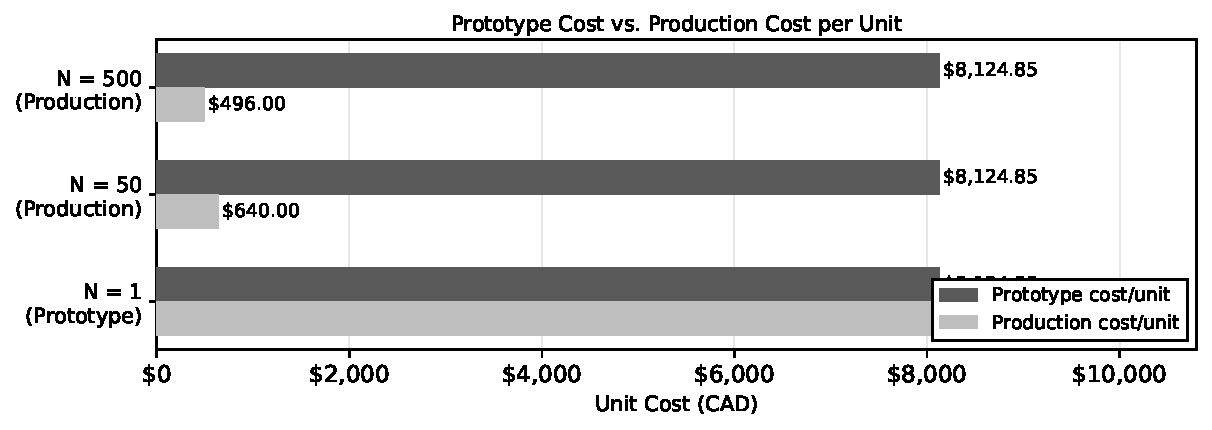
\includegraphics[width=0.85\textwidth]{images/fig_02_proto_vs_prod}
  \caption{Prototype cost per unit (\$8,124.85) compared with projected
           production cost at $N = 50$ (\$640) and $N = 500$ (\$496).
           The prototype cost is misleading as a production estimate: it
           bundles the full \$8,000 fixed cost onto a single unit.
           The dramatic reduction between $N = 1$ and $N = 50$ comes
           entirely from spreading that fixed cost across the run.}
  \label{fig:ch17-proto-vs-prod}
\end{figure}

Three observations follow directly from the figure.

\textit{First}, the largest cost reduction occurs between $N = 1$ and
$N = 50$: the unit cost falls by \$7,484.85, a reduction of 92\,\%.
The reduction from $N = 50$ to $N = 500$ is only \$144, a further
reduction of 22\,\%.
The curve is steep at low volume and flat at high volume, which is the
economic signature of Equation~\ref{eq:ch17-cunit}.

\textit{Second}, the prototype BOM cost (\$124.85) contributes less than
2\,\% of the \$8,124.85 prototype cost.
This means that even aggressive BOM reduction --- negotiating component
prices, substituting parts, redesigning for fewer line items --- cannot
materially reduce prototype cost; only spreading the fixed cost across
a larger $N$ can do that.

\textit{Third}, at $N = 500$ the unit cost of \$496 is only 3.3\,\% above
the \$480 variable-cost floor.
The product is approaching the asymptote: at this point further volume
increases yield diminishing returns, and attention should shift to
reducing $c_{\text{var}}$ itself --- through DFM/DFA improvements,
component consolidation, or a shift to a lower-cost assembly process.

% ─────────────────────────────────────────────────────────────────────────────
\section{Break-Even and Margin}
\label{sec:ch17-breakeven-margin}
% ─────────────────────────────────────────────────────────────────────────────

\subsection{Revenue Break-Even}
\label{sec:ch17-nbe}

Chapter~12 defined the \textbf{process break-even}\index{process break-even}
$N^{*} = 14.3 \to 15$~units as the volume at which 3D-printed and
injection-moulded housing costs are equal.
That is a manufacturing process decision.

This chapter uses a different break-even concept.
The \textbf{revenue break-even volume}\index{revenue break-even}
$N_{\text{be}}$ is the number of units that must be sold at price~$p$
to recover the fixed cost from the contribution margin on each sale.

Each unit sold at price $p$ contributes $(p - c_{\text{var}})$ toward
fixed-cost recovery.
Setting total contribution equal to fixed cost:

\begin{equation}
  N_{\text{be}} = \frac{C_{\text{fixed}}}{p - c_{\text{var}}}.
  \label{eq:ch17-nbe}
\end{equation}

For the sorting subsystem with $p = \$1{,}200$~CAD:
\[
  N_{\text{be}} = \frac{8{,}000}{1{,}200 - 480}
                = \frac{8{,}000}{720}
                = 11.11 \to 12\text{ units.}
\]

Twelve units sold at \$1,200 each generate \$14,400 in revenue; the
\$8,000 fixed cost is fully recovered, and the remaining \$6,400 covers
the variable cost of the run ($12 \times \$480 = \$5{,}760$, with \$640
profit).
Beyond the 12th unit, every additional sale generates \$720 of
\textbf{contribution margin}\index{contribution margin}.

Note that $N_{\text{be}} = 12$ (revenue break-even on sales) is different
from $N^{*} = 15$ (process break-even between manufacturing options).
These quantities answer different questions: $N_{\text{be}}$ tells you how
many units you must sell to stop losing money; $N^{*}$ tells you at which
volume to switch from 3D-printing to injection moulding.

\subsection{Gross Margin}
\label{sec:ch17-gm}

\textbf{Gross margin}\index{gross margin} (GM\%) measures the fraction of
selling price that remains after covering unit cost:
\[
  \text{GM}(N) = \frac{p - C_{\text{unit}}(N)}{p} \times 100\,\%.
\]

At $N = 50$:
\[
  \text{GM}(50) = \frac{1{,}200 - 640}{1{,}200}
               = \frac{560}{1{,}200} = 46.7\,\%.
\]

At $N = 500$:
\[
  \text{GM}(500) = \frac{1{,}200 - 496}{1{,}200}
                = \frac{704}{1{,}200} = 58.7\,\%.
\]

A gross margin of 46.7\,\% at $N = 50$ is commercially viable for a
hardware product in this category.
The improvement to 58.7\,\% at $N = 500$ confirms that the product becomes
more attractive economically as volume grows --- a key argument for the
Gate~3 go-decision.
Figure~\ref{fig:ch17-cost-projection} shows both margins annotated on the
unit-cost curve.

\subsection{Total Profit}
\label{sec:ch17-profit}

\textbf{Total profit}\index{total profit} (or contribution profit)
$\Pi(N)$ is the net gain after recovering both fixed and variable costs
from $N$ unit sales:

\begin{equation}
  \Pi(N) = N(p - c_{\text{var}}) - C_{\text{fixed}}.
  \label{eq:ch17-profit}
\end{equation}

The term $N(p - c_{\text{var}})$ is total contribution from all sales;
subtracting $C_{\text{fixed}}$ gives net profit after fixed-cost recovery.
Note that $\Pi(N_{\text{be}}) = 0$ by construction: the break-even volume
is the zero-profit point.

At $N = 500$:
\[
  \Pi(500) = 500 \times (1{,}200 - 480) - 8{,}000
           = 500 \times 720 - 8{,}000
           = 360{,}000 - 8{,}000
           = \$352{,}000\text{ CAD.}
\]

This figure --- \$352,000 profit on a run of 500 units --- is the economic
justification for the investment in Project~II.
It answers the gate committee's implicit question: ``If we fund the
development work required to reach production, is the payoff worth it?''

\subsection{Worked Example --- Full Projection for the Sorter}
\label{sec:ch17-worked}

The following calculation assembles all results in the order a Gate~3
reviewer would expect.
All inputs are locked values established in Chapters~11 and~12.

\medskip
\noindent\textbf{Given:}
\[
  C_{\text{fixed}} = \$8{,}000\text{ CAD},\quad
  c_{\text{var}}   = \$480\text{ CAD},\quad
  p                = \$1{,}200\text{ CAD},\quad
  C_{\text{BOM}}   = \$124.85\text{ CAD.}
\]

\medskip
\noindent\textbf{Step 1 --- Prototype cost per unit ($N = 1$):}
\[
  C_{\text{proto}} = C_{\text{BOM}} + C_{\text{fixed}}
                   = 124.85 + 8{,}000 = \$8{,}124.85\text{ CAD.}
\]

\noindent\textbf{Step 2 --- Unit cost at selected volumes
(Equation~\ref{eq:ch17-cunit}):}
\[
  C_{\text{unit}}(1)   = \frac{8{,}000}{1}   + 480 = 8{,}000 + 480
                        = \$8{,}480\text{ CAD.}
\]
\[
  C_{\text{unit}}(15)  = \frac{8{,}000}{15}  + 480 = 533.33 + 480
                        = \$1{,}013\text{ CAD (rounded).}
\]
\[
  C_{\text{unit}}(50)  = \frac{8{,}000}{50}  + 480 = 160 + 480
                        = \$640\text{ CAD.}
\]
\[
  C_{\text{unit}}(500) = \frac{8{,}000}{500} + 480 = 16 + 480
                        = \$496\text{ CAD.}
\]

\noindent\textbf{Step 3 --- Revenue break-even
(Equation~\ref{eq:ch17-nbe}):}
\[
  N_{\text{be}} = \frac{8{,}000}{1{,}200 - 480}
                = \frac{8{,}000}{720} = 11.11 \to 12\text{ units.}
\]

\noindent\textbf{Step 4 --- Gross margin:}
\[
  \text{GM}(50)  = \frac{1{,}200 - 640}{1{,}200} = \frac{560}{1{,}200}
                 = 46.7\,\%.
\]
\[
  \text{GM}(500) = \frac{1{,}200 - 496}{1{,}200} = \frac{704}{1{,}200}
                 = 58.7\,\%.
\]

\noindent\textbf{Step 5 --- Total profit at $N = 500$
(Equation~\ref{eq:ch17-profit}):}
\[
  \Pi(500) = 500 \times (1{,}200 - 480) - 8{,}000
           = 360{,}000 - 8{,}000 = \$352{,}000\text{ CAD.}
\]

\medskip
These five steps constitute the complete financial projection expected in a
Gate~3 submission.
Table~\ref{tab:ch17-summary} collects the results.

\begin{table}[htbp]
  \centering
  \caption{Cost projection summary for the IoT sorting subsystem
           ($C_{\text{fixed}} = \$8{,}000$, $c_{\text{var}} = \$480$,
           $p = \$1{,}200$~CAD).}
  \label{tab:ch17-summary}
  \begin{tabular}{lll}
    \hline
    Metric & Value & Equation \\
    \hline
    Prototype cost ($N = 1$)     & \$8{,}124.85 CAD & ---                          \\
    $C_{\text{unit}}(1)$         & \$8{,}480 CAD    & \ref{eq:ch17-cunit}          \\
    $C_{\text{unit}}(15)$        & \$1{,}013 CAD    & \ref{eq:ch17-cunit}          \\
    $C_{\text{unit}}(50)$        & \$640 CAD        & \ref{eq:ch17-cunit}          \\
    $C_{\text{unit}}(500)$       & \$496 CAD        & \ref{eq:ch17-cunit}          \\
    Revenue break-even $N_{\text{be}}$  & 12 units  & \ref{eq:ch17-nbe}            \\
    Gross margin at $N = 50$     & 46.7\,\%         & ---                          \\
    Gross margin at $N = 500$    & 58.7\,\%         & ---                          \\
    Total profit $\Pi(500)$      & \$352{,}000 CAD  & \ref{eq:ch17-profit}         \\
    \hline
  \end{tabular}
\end{table}

\begin{figure}[htbp]
  \centering
  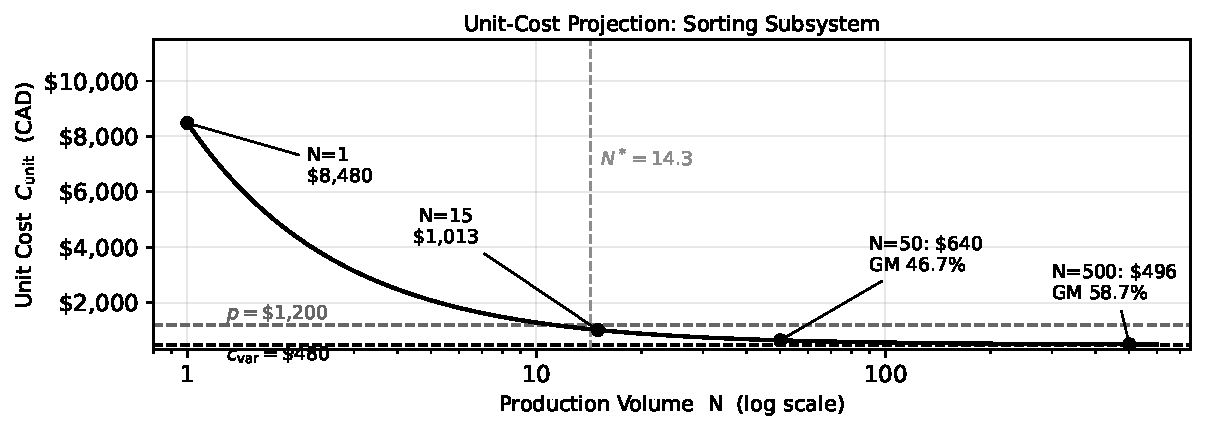
\includegraphics[width=0.85\textwidth]{images/fig_01_cost_projection}
  \caption{$C_{\text{unit}}(N)$ for the IoT sorting subsystem on a log
           $N$-axis.
           The curve falls from \$8,480 at $N = 1$ to \$496 at $N = 500$,
           asymptoting to $c_{\text{var}} = \$480$ (lower dashed line).
           The selling price $p = \$1{,}200$ is marked by the upper dashed
           line; the vertical dashed line at $N^* = 14.3$ is the
           process break-even from Chapter~12.
           Annotated arrows show gross margin at $N = 50$ (46.7\,\%) and
           $N = 500$ (58.7\,\%).}
  \label{fig:ch17-cost-projection}
\end{figure}

% ─────────────────────────────────────────────────────────────────────────────
\section{Extrinsic Value and Gate~3 Readiness}
\label{sec:ch17-gate3}
% ─────────────────────────────────────────────────────────────────────────────

A Gate~3 review evaluates two distinct questions: what the prototype
\emph{proved} about the design, and what \emph{remains} unresolved before
production can begin.
A team that can answer both questions clearly --- with quantitative evidence
for the first and a prioritised list for the second --- demonstrates the
engineering judgment that distinguishes a credible Gate~3 submission from a
demonstration of a working prototype.

\subsection{What the Prototype Proved}
\label{sec:ch17-proved}

The sorting subsystem prototype addressed the five primary unknowns
identified at Gate~1 (Chapter~4) and tracked through the Stage-Gate
process.

\begin{enumerate}
  \item \textbf{Sort accuracy and latency.}\index{sort accuracy}
        Acceptance testing (Chapter~14) demonstrated a mean sort latency of
        99.06~ms against a specification of $\leq 100$~ms, with a process
        capability index $C_p = 1.73$.
        The system meets specification with substantial margin.

  \item \textbf{Battery life and power budget.}\index{power budget}
        The validated power budget predicts a battery life of 50.5~days
        on the specified cell, exceeding the 30-day requirement by 68\,\%.

  \item \textbf{Structural integrity.}\index{structural integrity}
        The bracket safety factor is $\text{SF} = 5.29$, well above the
        $\text{SF} \geq 2$ requirement established in Chapter~4.

  \item \textbf{AI inference end-to-end.}\index{AI inference}
        The on-device ML model runs inference end-to-end on the target
        microcontroller, meeting latency requirements without cloud
        connectivity.

  \item \textbf{BOM cost and sourcing.}\index{BOM cost}
        The costed BOM from Chapter~11 is \$124.85~CAD per prototype unit,
        with all components sourced from qualified distributors.
        All components are in active production with verified lead times.
\end{enumerate}

\subsection{What Remains for Project~II}
\label{sec:ch17-remains}

Six items are explicitly out of scope for Project~I and constitute the
primary risk items that Project~II must resolve.

\begin{enumerate}
  \item \textbf{Production-grade firmware.}\index{production firmware}
        The prototype firmware does not support over-the-air (OTA) updates.
        Field deployment at scale requires a validated OTA update mechanism;
        without it, firmware defects discovered post-deployment require a
        physical service call.

  \item \textbf{Regulatory certification.}\index{regulatory certification}
        The prototype has not been submitted to FCC or ISED (Innovation,
        Science and Economic Development Canada) for wireless emissions
        testing.
        Certification is mandatory before commercial sale in Canada and the
        United States and represents a fixed cost of \$8,000--\$15,000 plus
        12--20 weeks of test time.

  \item \textbf{Injection-moulded housing.}\index{injection moulding}
        The prototype housing is FDM-printed.
        The process break-even analysis from Chapter~12 identified
        $N^* = 14.3 \to 15$~units as the transition point; above 15~units,
        an injection-moulded housing is more cost-effective.
        The mould tool must be designed, cut, and validated before production
        begins.

  \item \textbf{Supply-chain qualification.}\index{supply-chain qualification}
        Prototype components were purchased at retail from distributors.
        Production requires negotiated pricing, lead-time agreements, and
        approved vendor lists for all critical components.

  \item \textbf{Cost reduction to below $N_{\text{be}} = 12$.}\index{cost reduction}
        The current model assumes $c_{\text{var}} = \$480$ at volume.
        Achieving the projected margins requires that BOM negotiation and
        DFM/DFA improvements deliver this variable cost; the prototype does
        not validate production pricing.

  \item \textbf{Customer pilot program.}\index{customer pilot}
        No customer has operated the system in a field environment.
        A pilot with 3--5 units in customer hands is essential to validate
        the 30-day battery-life claim and to surface firmware edge cases that
        do not appear in laboratory testing.
\end{enumerate}

\subsection{Gate~3 Readiness Statement}
\label{sec:ch17-readiness-statement}

The \textbf{Gate~3 readiness statement}\index{Gate~3 readiness statement}
is a two-to-three sentence executive summary that the gate committee reads
before examining any supporting data.
It must state what was proved (with quantitative evidence), what remains
unresolved, and why proceeding is justified.

For the sorting subsystem:

\begin{quote}
  The robotic sorting subsystem has demonstrated sort accuracy within
  specification (mean latency 99.06~ms, $C_p = 1.73$), battery life
  exceeding 50~days, and structural safety factor $\text{SF} = 5.29$.
  The design is ready for Project~II, which will address
  production-scale firmware, regulatory certification, and supply-chain
  qualification.
\end{quote}

% ─────────────────────────────────────────────────────────────────────────────
\section{Lessons Learned}
\label{sec:ch17-lessons}
% ─────────────────────────────────────────────────────────────────────────────

An honest lessons-learned section is among the most valuable outputs of
Project~I.
Gate committees distrust teams that claim everything went according to plan;
they trust teams that can identify what went wrong, explain why, and
articulate what they would do differently.
The following observations reflect the specific experience of the sorting
subsystem project.

\textbf{What the team would do differently.}
\begin{enumerate}
  \item \textit{Component lead time.} Two components on the BOM had 14-week
        lead times that were not identified until procurement began in
        Chapter~11.
        Future projects should run lead-time screening in parallel with
        component selection (Chapter~6), not after it.

  \item \textit{Firmware version control.} The first six weeks of firmware
        development used informal file naming ($\texttt{main\_v2\_FINAL.c}$,
        $\texttt{main\_v2\_FINAL\_fixed.c}$) rather than the Git workflow
        formalised in Chapter~13.
        Three hours were lost reconstructing a working build that had been
        overwritten.
        Version control should be the first task on Day~1, not an
        afterthought at Gate~3.

  \item \textit{Structural analysis timing.} The bracket FEA (Chapter~9)
        was performed after the housing geometry was frozen.
        When the initial FEA flagged an under-thickness rib, the CAD model
        required revision, which propagated to the print file, the assembly
        drawing, and the test fixture.
        Structural analysis should be embedded in the design-review cadence,
        not deferred to a single milestone.
\end{enumerate}

\textbf{Assumptions that proved wrong.}
\begin{enumerate}
  \item The initial power budget assumed the microcontroller would spend
        85\,\% of its time in deep sleep.
        Profiling revealed the actual sleep fraction was 71\,\% due to
        interrupt latency from the sensor polling loop.
        The revised budget still cleared the 30-day specification, but the
        assumption was wrong and the team was fortunate the margin was large.

  \item The team estimated that AI model training would require one week.
        Data collection, labelling, augmentation, and validation took three
        weeks.
        Any project involving a trained ML model should budget at least
        twice the time estimated for the data pipeline.
\end{enumerate}

\textbf{One result that was better than expected.}
The sort accuracy specification ($\leq 100$~ms mean latency) was set
conservatively based on an early literature survey.
After implementation the measured mean was 99.06~ms with $C_p = 1.73$,
far better than the team expected from a first-pass firmware implementation.
The margin is large enough that Project~II can allocate computational
budget to OTA update handling without revisiting the latency specification.

% ─────────────────────────────────────────────────────────────────────────────
\section{The Handoff to Project~II}
\label{sec:ch17-handoff}
% ─────────────────────────────────────────────────────────────────────────────

Figure~\ref{fig:ch17-gate3-readiness} presents the Gate~3 readiness
assessment as a structured two-column view.
The left column records what Project~I delivers as validated artefacts.
The right column records what Project~II must resolve before production can
begin.
Neither column is a list of successes and failures: every item in the right
column is a \emph{scoped risk} with a known resolution path.

\begin{figure}[htbp]
  \centering
  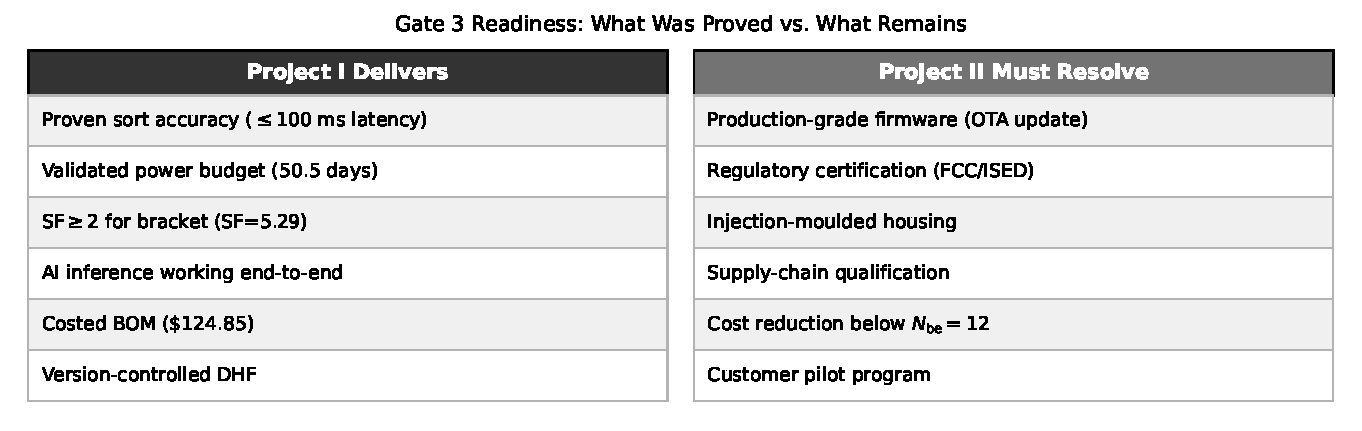
\includegraphics[width=0.85\textwidth]{images/fig_03_gate3_readiness}
  \caption{Gate~3 readiness matrix for the sorting subsystem.
           Left: deliverables that Project~I provides as validated artefacts.
           Right: unresolved items that Project~II must address before
           production.
           Every item in the right column has a known resolution path,
           cost estimate, and schedule implication.}
  \label{fig:ch17-gate3-readiness}
\end{figure}

The six Project~I deliverables in the left column correspond directly to
the Gate~3 acceptance criteria established in Chapter~4 and tested in
Chapter~14.
Every item is supported by a quantitative test result, a signed test report,
and a version-controlled entry in the Design History File.

The six Project~II items in the right column are not failures.
They are engineering tasks that were deliberately deferred because completing
them during Project~I would have consumed schedule and budget without
reducing the primary unknowns.
A firmware OTA update mechanism is meaningless before the firmware itself
is validated.
An injection-mould tool is an unnecessary capital expenditure before the
housing geometry is frozen by test data.
The sequence --- prototype, validate, then invest in production tooling ---
is the Stage-Gate model working as designed.

\paragraph{In Practice.}
``It works'' does not mean ``ready to produce.''
The economic gap between a working prototype and a manufacturable product
is often larger than the engineering gap.
Regulatory certification, supply-chain qualification, and production-grade
firmware can each consume as much time and money as the prototype development
itself.
A Gate~3 submission that acknowledges this gap with a specific list of
Project~II tasks is more credible, not less credible, than one that claims
the product is production-ready.
Gate committees have seen enough optimistic Gate~3 presentations to
recognise the ones where the team has done the work to understand what they
do not yet know.

\paragraph{Common Pitfalls.}
\label{sec:ch17-pitfalls}

Two specific errors recur in Gate~3 submissions.

\begin{enumerate}
  \item \textbf{``It works'' is treated as equivalent to ``ready to
        produce.''}\index{it works fallacy}
        A prototype that meets its functional specification is a validated
        design, not a production design.
        The gap between the two includes regulatory certification, supply-chain
        qualification, production-grade firmware, manufacturability at volume,
        and field reliability under conditions that were not tested in the
        laboratory.
        Teams that present a working prototype and a unit-cost calculation
        without addressing these items have not completed a Gate~3 submission;
        they have completed a science-fair demonstration.

  \item \textbf{A negative economic finding is treated as a failure.}
        If the break-even analysis shows $N_{\text{be}} = 12$~units but the
        total addressable market is only 8~units, that is not a failed project
        --- it is a project whose scope must change.
        Options include: reducing $C_{\text{fixed}}$ (a simpler test fixture,
        a less complex mould tool), reducing $c_{\text{var}}$ (BOM
        renegotiation, assembly simplification), raising $p$ (moving
        upmarket, adding features that justify a higher price), or exiting
        the market and licensing the technology.
        The Gate~3 recommendation in this case is not ``proceed'' or ``kill''
        but ``proceed with revised scope.''
        A team that presents this analysis honestly, with options evaluated,
        demonstrates exactly the economic judgment that a gate committee is
        looking for.
\end{enumerate}

% ─────────────────────────────────────────────────────────────────────────────
\section*{Try It Yourself}
\addcontentsline{toc}{section}{Try It Yourself}
\label{sec:ch17-try}
% ─────────────────────────────────────────────────────────────────────────────

A student team has developed a motion-sensor module with the following
cost parameters:
\[
  p = \$380\text{ CAD},\quad
  c_{\text{var}} = \$95\text{ CAD},\quad
  C_{\text{fixed}} = \$4{,}500\text{ CAD.}
\]

\begin{enumerate}
  \item[(a)] Using Equation~\ref{eq:ch17-cunit}, compute $C_{\text{unit}}$
        at $N = 25$, $N = 100$, and $N = 1{,}000$.
        Show every arithmetic step.

  \item[(b)] Using Equation~\ref{eq:ch17-nbe}, compute $N_{\text{be}}$.
        How many units must be sold to recover the fixed cost?

  \item[(c)] Compute GM\% at $N = 100$ and $N = 1{,}000$.

  \item[(d)] Using Equation~\ref{eq:ch17-profit}, compute $\Pi(200)$.
        Write a one-sentence Gate~3 readiness statement assuming all
        functional tests passed at specification.
\end{enumerate}

% ─────────────────────────────────────────────────────────────────────────────
\section*{Review Questions}
\addcontentsline{toc}{section}{Review Questions}
\label{sec:ch17-review}
% ─────────────────────────────────────────────────────────────────────────────

\begin{enumerate}
  \item \textbf{(Conceptual)} Explain why the unit cost of a single prototype
        is a misleading cost estimate for a production product.
        What two cost components does $C_{\text{unit}}(N)$
        (Equation~\ref{eq:ch17-cunit}) correctly separate?

  \item \textbf{(Conceptual)} A team's economic analysis shows that
        break-even requires 200~units but the total addressable market is
        150~units.
        Is this a failure?
        Explain what options remain and what the Gate~3 recommendation
        should be.

  \item \textbf{(Applied, calculation)} A product: $p = \$520$~CAD,
        $c_{\text{var}} = \$180$~CAD, $C_{\text{fixed}} = \$6{,}200$~CAD.
        Compute $C_{\text{unit}}$ at $N = 20$, $N = 100$, and $N = 500$.
        Compute $N_{\text{be}}$.
        Compute GM\% at $N = 100$.
        (Use Equations~\ref{eq:ch17-cunit} and~\ref{eq:ch17-nbe}.)

  \item \textbf{(Applied, calculation)} Using the values from Q3, compute
        $\Pi(300)$.
        Then compute $\Pi(50)$.
        Interpret both results.
        (Use Equation~\ref{eq:ch17-profit}.)

  \item \textbf{(Applied, multi-step)} A wearable device:
        $p = \$890$~CAD, $c_{\text{var}} = \$310$~CAD,
        $C_{\text{fixed}} = \$12{,}000$~CAD, $C_{\text{BOM}} = \$310$~CAD
        (1~unit).
        Compute:
        \begin{enumerate}
          \item[(a)] Prototype cost per unit.
          \item[(b)] $C_{\text{unit}}$ at $N = 30$ using
                Equation~\ref{eq:ch17-cunit}.
          \item[(c)] $N_{\text{be}}$ using Equation~\ref{eq:ch17-nbe}.
          \item[(d)] GM\% at $N = 30$.
          \item[(e)] $\Pi(100)$ using Equation~\ref{eq:ch17-profit}.
        \end{enumerate}
        Write a two-sentence Gate~3 readiness statement assuming functional
        tests passed.
\end{enumerate}

% ─────────────────────────────────────────────────────────────────────────────
\section*{Portfolio Entry}
\addcontentsline{toc}{section}{Portfolio Entry}
\label{sec:ch17-portfolio}
% ─────────────────────────────────────────────────────────────────────────────

This is the final submission of your prototype documentation package and
your Gate~3 presentation.

\textbf{Documentation package.}
Submit the complete portfolio assembled in Chapter~16, updated with the
following additions from this chapter:

\begin{enumerate}
  \item[(a)] \textit{Cost projection} --- a parameter table
        ($C_{\text{fixed}}$, $c_{\text{var}}$, $p$, $Y$) with sources,
        and a unit-cost table showing $C_{\text{unit}}$ at $N = 50$,
        $N = 100$, and $N = 500$ with corresponding GM\%.

  \item[(b)] \textit{Gate~3 readiness statement} --- two to three sentences
        stating what the prototype proved, what remains unresolved, and
        why proceeding to Project~II is justified.

  \item[(c)] \textit{Lessons learned} --- one page: three things the team
        would do differently, two assumptions that proved wrong, and one
        result that was better than expected.
\end{enumerate}

\textbf{Final presentation.}
Deliver a 10--15~minute live presentation demonstrating your prototype
against the Gate~3 acceptance criteria.
The presentation must cover:

\begin{enumerate}
  \item[(d)] \textit{Prototype demonstration} --- live or recorded
        demonstration of the prototype meeting its primary specification.

  \item[(e)] \textit{Test results summary} --- key quantitative results
        from Chapter~14 with pass/fail decision against acceptance criteria.

  \item[(f)] \textit{Production economics} --- the cost projection and
        break-even analysis from this chapter.

  \item[(g)] \textit{Gate~3 readiness statement} --- delivered verbally,
        supported by the figure from \S\ref{sec:ch17-handoff}.
\end{enumerate}

The documentation package and presentation together constitute
\textbf{Milestone~3}\index{Milestone~3} --- the Gate~3 submission that
closes Project~I and opens the path to Project~II.

% ─────────────────────────────────────────────────────────────────────────────
\section*{Chapter Summary}
\addcontentsline{toc}{section}{Chapter Summary}
\label{sec:ch17-summary}
% ─────────────────────────────────────────────────────────────────────────────

This chapter completes the arc that began in Chapter~1 with a sorting
problem and a blank Stage-Gate chart.
Over sixteen chapters the project moved from an open question (``can a
robotic subsystem sort objects reliably under battery power?'') through
specifications, architecture, component selection, DFM review, BOM
procurement, version control, AI integration, structural analysis,
power budgeting, validation testing, intellectual property strategy, and
documentation assembly.
This final chapter added the economic dimension: the unit-cost curve,
the revenue break-even at 12~units, gross margins of 46.7\,\% and 58.7\,\%
at volumes of 50 and 500, and a total profit of \$352,000 at volume~500.

The equations that produced these numbers --- Equations~\ref{eq:ch17-cunit},
\ref{eq:ch17-nbe}, and~\ref{eq:ch17-profit} --- are not complex.
The discipline is not in the mathematics; it is in the honesty required to
apply them.
A team that uses prototype cost as a production cost estimate, that omits
regulatory certification from the fixed-cost budget, or that treats a
working prototype as a production-ready product has not completed the work
this chapter requires.

A Gate~3 submission is not a finished product.
It is a structured argument, supported by quantitative evidence, that the
risk of proceeding to Project~II is lower than the risk of stopping.
The sorting subsystem prototype demonstrated sort accuracy within
specification, battery life well above requirement, and structural margins
that exceed the safety factor by a factor of 2.6.
The economic model shows break-even at 12~units and a \$352,000 profit at
volume~500.
Six specific items have been identified for Project~II, each with a known
resolution path.

That is what a Gate~3 submission looks like.
Not a claim that everything is solved --- but evidence that enough is known
to justify the next investment, and enough honesty to say exactly what
is not yet known.
The risk of proceeding is quantified.
The risk of stopping --- foregoing \$352,000 in potential profit and
abandoning a technically validated design --- is now the higher risk.
That is the economic argument for opening Project~II.
